% Options for packages loaded elsewhere
\PassOptionsToPackage{unicode}{hyperref}
\PassOptionsToPackage{hyphens}{url}
%
\documentclass[
  10pt,
  a4paper,
]{article}
\usepackage{amsmath,amssymb}
\usepackage{iftex}
\ifPDFTeX
  \usepackage[T1]{fontenc}
  \usepackage[utf8]{inputenc}
  \usepackage{textcomp} % provide euro and other symbols
\else % if luatex or xetex
  \usepackage{unicode-math} % this also loads fontspec
  \defaultfontfeatures{Scale=MatchLowercase}
  \defaultfontfeatures[\rmfamily]{Ligatures=TeX,Scale=1}
\fi
\usepackage{lmodern}
\ifPDFTeX\else
  % xetex/luatex font selection
  \setmainfont[]{DejaVu Sans}
  \setmonofont[]{DejaVu Sans Mono}
\fi
% Use upquote if available, for straight quotes in verbatim environments
\IfFileExists{upquote.sty}{\usepackage{upquote}}{}
\IfFileExists{microtype.sty}{% use microtype if available
  \usepackage[]{microtype}
  \UseMicrotypeSet[protrusion]{basicmath} % disable protrusion for tt fonts
}{}
\makeatletter
\@ifundefined{KOMAClassName}{% if non-KOMA class
  \IfFileExists{parskip.sty}{%
    \usepackage{parskip}
  }{% else
    \setlength{\parindent}{0pt}
    \setlength{\parskip}{6pt plus 2pt minus 1pt}}
}{% if KOMA class
  \KOMAoptions{parskip=half}}
\makeatother
\usepackage{xcolor}
\usepackage[margin=19mm]{geometry}
\usepackage{longtable,booktabs,array}
\usepackage{calc} % for calculating minipage widths
% Correct order of tables after \paragraph or \subparagraph
\usepackage{etoolbox}
\makeatletter
\patchcmd\longtable{\par}{\if@noskipsec\mbox{}\fi\par}{}{}
\makeatother
% Allow footnotes in longtable head/foot
\IfFileExists{footnotehyper.sty}{\usepackage{footnotehyper}}{\usepackage{footnote}}
\makesavenoteenv{longtable}
\usepackage{graphicx}
\makeatletter
\def\maxwidth{\ifdim\Gin@nat@width>\linewidth\linewidth\else\Gin@nat@width\fi}
\def\maxheight{\ifdim\Gin@nat@height>\textheight\textheight\else\Gin@nat@height\fi}
\makeatother
% Scale images if necessary, so that they will not overflow the page
% margins by default, and it is still possible to overwrite the defaults
% using explicit options in \includegraphics[width, height, ...]{}
\setkeys{Gin}{width=\maxwidth,height=\maxheight,keepaspectratio}
% Set default figure placement to htbp
\makeatletter
\def\fps@figure{htbp}
\makeatother
\setlength{\emergencystretch}{3em} % prevent overfull lines
\providecommand{\tightlist}{%
  \setlength{\itemsep}{0pt}\setlength{\parskip}{0pt}}
\setcounter{secnumdepth}{-\maxdimen} % remove section numbering
\ifLuaTeX
\usepackage[bidi=basic]{babel}
\else
\usepackage[bidi=default]{babel}
\fi
\babelprovide[main,import]{french}
\ifPDFTeX
\else
\babelfont{rm}[]{DejaVu Sans}
\fi
% get rid of language-specific shorthands (see #6817):
\let\LanguageShortHands\languageshorthands
\def\languageshorthands#1{}
\usepackage{etoolbox}
\usepackage{microtype}
\usepackage{float}
\floatplacement{figure}{H}
\sloppy
\setlength{\emergencystretch}{5em}
\AtBeginEnvironment{longtable}{\small}
\ifLuaTeX
  \usepackage{selnolig}  % disable illegal ligatures
\fi
\IfFileExists{bookmark.sty}{\usepackage{bookmark}}{\usepackage{hyperref}}
\IfFileExists{xurl.sty}{\usepackage{xurl}}{} % add URL line breaks if available
\urlstyle{same}
\hypersetup{
  pdftitle={Weil : retrouver la piste du signe global},
  pdfauthor={Vincent P. P. NOËL - dossier de recherche, rédaction assistée},
  pdflang={fr-FR},
  hidelinks,
  pdfcreator={LaTeX via pandoc}}

\title{Weil : retrouver la piste du signe global}
\usepackage{etoolbox}
\makeatletter
\providecommand{\subtitle}[1]{% add subtitle to \maketitle
  \apptocmd{\@title}{\par {\large #1 \par}}{}{}
}
\makeatother
\subtitle{Programme Riemann - V6.51 - Document 76}
\author{Vincent P. P. NOËL - dossier de recherche, rédaction assistée}
\date{13 octobre 2026}

\begin{document}
\maketitle

{
\setcounter{tocdepth}{2}
\tableofcontents
}
\textbf{Conclusion de la reconstruction.} La piste la mieux attestée à
remettre au centre est la compensation \textbf{signée} du document 70.
Elle n'avait pas été réfutée. Les documents suivants ont surtout
développé des enveloppes et des certificats locaux. Cette évolution est
une bifurcation de méthode ; les traces ne permettent pas d'affirmer
qu'une preuve globale avait été découverte puis perdue.

Trois constructions nouvelles donnent un sens précis à sa reprise :
traiter la dette dans le dual de la norme d'énergie ; remplacer une
liste de supports par une grammaire de paquets traduits et de matrices
Toeplitz. La première allège une obligation de régularité. La seconde
incorpore le signe et la couverture dans une seule famille structurée.
Enfin, deux filtres premiers engendrent densément les tests polaires.
Leur loi arithmétique universelle reste à démontrer.

\hypertarget{comment-lire-les-provenances}{%
\subsection{Comment lire les
provenances}\label{comment-lire-les-provenances}}

\begin{itemize}
\tightlist
\item
  \textbf{{[}T{]} Trace antérieure} : conversation visible et documents
  67 à 74 conservés dans le ZIP V6.49. Une preuve écrite dans le dossier
  n'est pas une validation publiée.
\item
  \textbf{{[}R{]} Reconstruction} : construction ou implication
  explicitée pour cette enquête. Elle n'est pas attribuée à un
  raisonnement interne retrouvé.
\item
  \textbf{{[}P{]} Reprise postérieure} : document 75 et calculs V6.50,
  conservés comme résultats locaux ; ils ne déterminent pas
  automatiquement le choix de la piste.
\item
  \textbf{{[}L{]} Littérature} : énoncé vérifié dans une source primaire
  citée en fin de note.
\end{itemize}

Les statuts sont distincts de ces provenances : \textbf{démontré dans le
dossier}, \textbf{conditionnel}, \textbf{hypothèse de travail},
\textbf{spéculation}, \textbf{méthode réfutée}. L'absence d'un artefact
postérieur à V6.49 n'établit pas ce qui aurait été pensé pendant
l'interruption. Cette enquête reconstruit des programmes de recherche
publics et vérifiables à partir de leurs traces.

\begin{figure}
\centering
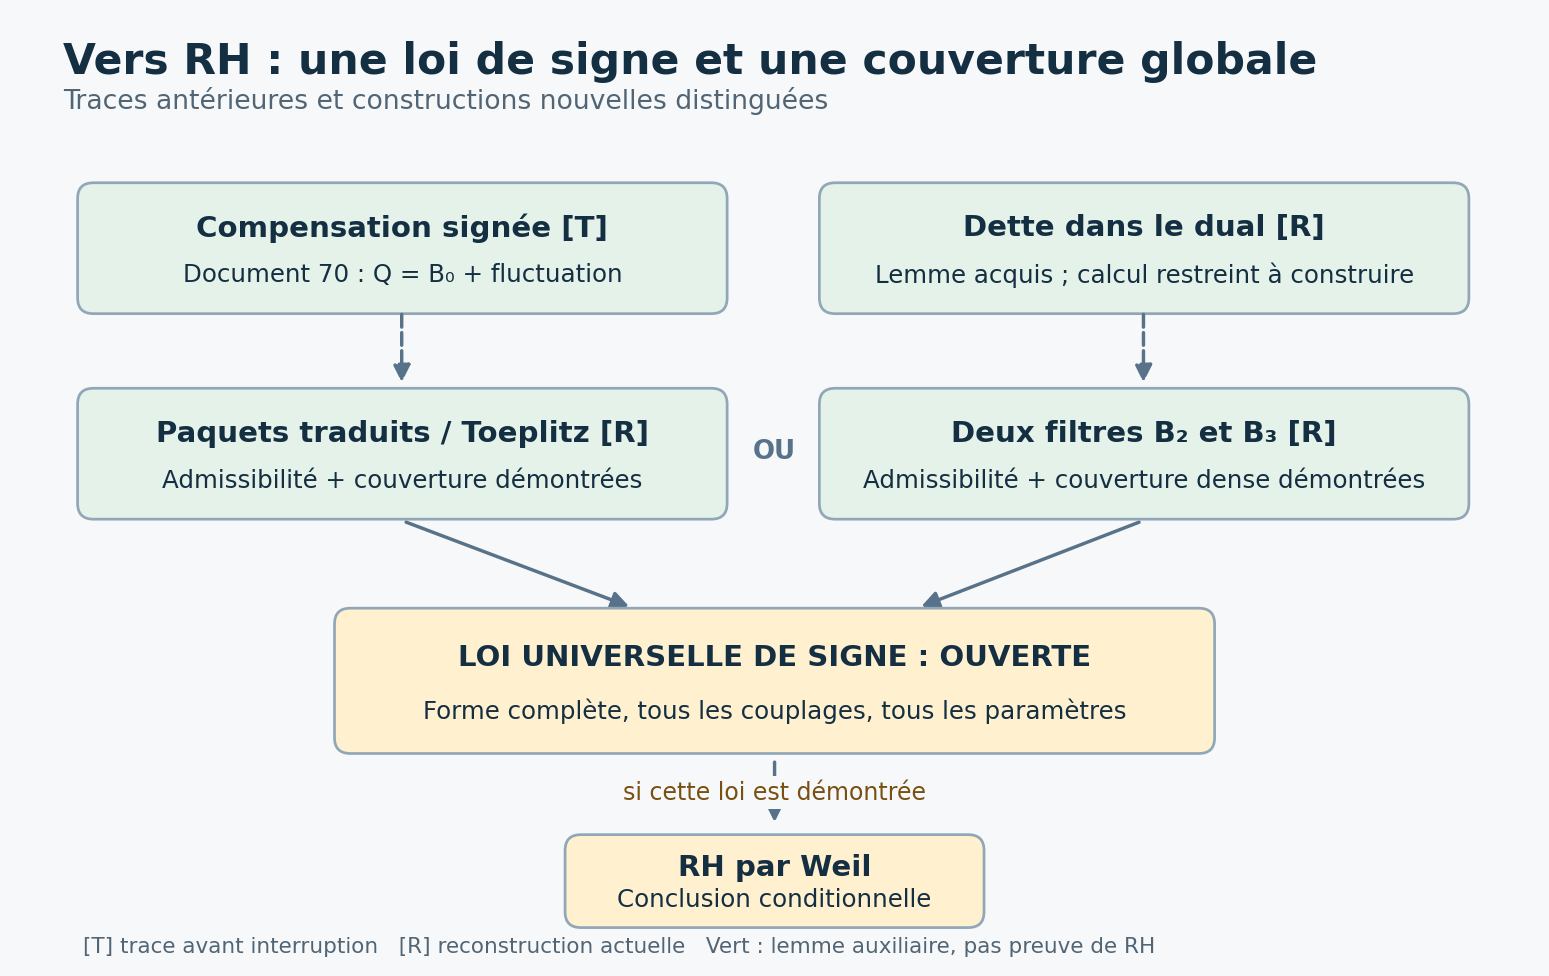
\includegraphics[width=1\textwidth,height=\textheight]{76_CARTE_PISTES_GLOBALES.png}
\caption{Deux grammaires couvrantes ; la loi universelle de signe reste
ouverte.}
\end{figure}

\hypertarget{hypothuxe8ses-initiales-et-questions-ouvertes}{%
\section{1. Hypothèses initiales et questions
ouvertes}\label{hypothuxe8ses-initiales-et-questions-ouvertes}}

\hypertarget{le-but-global-est-connu}{%
\subsection{1.1. Le but global est
connu}\label{le-but-global-est-connu}}

\textbf{{[}T, L{]}} Nous cherchons le signe de la forme complète de
Weil, pour tout test compact admissible. Ce qui demeure inconnu est le
mécanisme qui impose ce signe. La destination n'est donc pas un point
indéfini du labyrinthe.

Pour \(S>0\), les fonctions sont prolongées par zéro hors de \([-S,S]\).
Posons \[
\ell_\pm(f)=\int_{\mathbb R}f(x)e^{\pm x/2}\,dx,\qquad
m(f)=\|f\|_2^2.
\] \[
\mathcal E(f)=\int_{\mathbb R}a(t)|\widehat f(t)|^2\,dt,\qquad
R(f)=m(f)+\mathcal E(f),
\] \[
a(t)=\sum_{n\ge0}\frac{2t^2}{b_n(b_n^2+t^2)},\qquad b_n=2n+\tfrac12.
\] La Fourier est unitaire. L'espace \(X_S\) impose support, moments
nuls et énergie finie. Pour \(q=p^j\), écrire \(d_q=\log q\),
\(c_q=\log p/\sqrt q\). Alors \[
h_f(d)=\int f(x)\overline{f(x-d)}\,dx,
\] \[
\boxed{Q_W(f)=\mathcal E(f)-C_0m(f)
-2\sum_{d_q<2S}c_q\Re h_f(d_q)},\qquad
C_0=\log(8\pi)+\gamma_E+\pi/2.
\] La somme est finie pour chaque support. Au seuil \(d_q=2S\), la
corrélation est nulle presque partout. Les tests sont complexes ; une
vérification sur quelques fonctions réelles ne les remplace pas.

Connes-Consani, équation (4) et proposition C.1, autorisent les deux
annulations polaires dans le critère de Weil. Avec cette normalisation,
\[
\boxed{\mathrm{RH}\ \Longleftrightarrow\
Q_W(f)\ge0\quad\text{pour tout test compact admissible}.}
\] Les unités fictives du corpus sont cohérentes : amplitude pour \(f\),
amplitude au carré pour \(m,\mathcal E,R,Q_W\). Elles contrôlent les
formules, pas leur signe.

\hypertarget{les-quatre-portes-relues-globalement}{%
\subsection{1.2. Les quatre portes, relues
globalement}\label{les-quatre-portes-relues-globalement}}

\begin{longtable}[]{@{}
  >{\raggedright\arraybackslash}p{(\columnwidth - 4\tabcolsep) * \real{0.3333}}
  >{\raggedright\arraybackslash}p{(\columnwidth - 4\tabcolsep) * \real{0.3333}}
  >{\raggedright\arraybackslash}p{(\columnwidth - 4\tabcolsep) * \real{0.3333}}@{}}
\toprule\noalign{}
\begin{minipage}[b]{\linewidth}\raggedright
Porte
\end{minipage} & \begin{minipage}[b]{\linewidth}\raggedright
Trace acquise avant interruption
\end{minipage} & \begin{minipage}[b]{\linewidth}\raggedright
Obligation restante
\end{minipage} \\
\midrule\noalign{}
\endhead
\bottomrule\noalign{}
\endlastfoot
Arithmétique & Annulation polaire ; fluctuation exacte ; phases
\(z_{p^j}=z_p^j\) & Compensation signée du bilan complet, avec les
couplages \\
Tête et queue & Énergie logarithmique ; réduction identité moins compact
; budgets de queue & Une tête et une dette contrôlables pour une famille
non bornée \\
Couplages & Schur exact ; majorant par Gram de résidus L² & Normes des
résidus requises par la méthode réellement choisie \\
Couverture & Contrats à support fixé ; familles admissibles denses &
Preuve pour des supports arbitrairement grands, ou grammaire couvrante
équivalente \\
\end{longtable}

\textbf{{[}P{]}} Le certificat V6.50 atteint \(S=11/20\) dans son modèle
arithmétique déclaré ; son transport conserve les moments et contrôle
les normes. Ce sont des résultats locaux utiles. Le transport ne
conserve pas automatiquement le signe.

\textbf{{[}T{]}} Les branches de zéros, collisions doubles et
coefficient complexe arbitraire restent des problèmes propres. Le
critère de Weil offre une voie à RH qui n'exige pas de suivre chaque
zéro ni de prouver leur simplicité.

\hypertarget{plusieurs-trajectoires-plausibles}{%
\section{2. Plusieurs trajectoires
plausibles}\label{plusieurs-trajectoires-plausibles}}

\hypertarget{reprendre-la-fluctuation-signuxe9e-apruxe8s-annulation-polaire}{%
\subsection{2.1. Reprendre la fluctuation signée après annulation
polaire}\label{reprendre-la-fluctuation-signuxe9e-apruxe8s-annulation-polaire}}

\textbf{{[}T : document 70, sections 3 à 5 et 9{]}} Avec
\(P=\partial_x^2-1/4\), \(f=P\psi\) est admissible pour une graine lisse
compacte. Posons \[
P_0(f)=\int\frac{|\widehat f(t)|^2}{t^2+1/4}\,dt
=\|\psi'\|_2^2+\tfrac14\|\psi\|_2^2.
\] L'identité polaire donne exactement \[
2\int_0^{2S}e^{u/2}\Re h_f(u)\,du=-P_0(f).
\] Avec \(\Psi(x)=\sum_{p^j\le x}\log p\) et
\(\Delta_\Psi(u)=\Psi(e^u)-e^u+1\), on obtient \[
\boxed{Q_W=B_0+\mathfrak F_\Psi},\qquad
B_0=\mathcal E-C_0m+P_0,
\] \[
\mathfrak F_\Psi(f)=2\int_0^{2S}\Delta_\Psi(u)e^{-u/2}
\left(H_f'(u)-\tfrac12H_f(u)\right)du,\quad H_f=\Re h_f.
\] Cette dernière écriture exige \(H^1\). Sur \(X_S\), l'écriture de
Stieltjes sans dériver la corrélation conserve l'identité. Aucun bord
n'est omis.

Le document 70 démontre que \(B_0(Pw_S)<0\)pour tout\(S\ge16\), avec
\(w_S(x)=(1-x^2/S^2)^4\) sur la boîte. Une famille lisse étirée donne
aussi \(B_0/m\to4-C_0<0\). La fluctuation doit donc réparer un déficit
effectif. La stratégie qui la traiterait comme une petite erreur perd
cette obligation.

\textbf{{[}R : programme à rouvrir{]}} Identifier les directions où
\(B_0\) est dangereux, puis établir une estimation signée qui conserve
leur interaction avec le complément. La seule inégalité
\(\mathfrak F_\Psi\ge-B_0\) serait un renommage du but : il faut une
identité, une factorisation ou une estimation arithmétique indépendante
qui la démontre sur une famille complète.

\hypertarget{traiter-la-dette-dans-le-dual-de-luxe9nergie}{%
\subsection{2.2. Traiter la dette dans le dual de
l'énergie}\label{traiter-la-dette-dans-le-dual-de-luxe9nergie}}

\textbf{{[}T{]}} Le document 70 donne un certificat suffisant utilisant
les sources fortes en L² et avertit que sa convergence peut demander une
norme de graphe.

\textbf{{[}R : proposition démontrée ci-dessous{]}} Cette régularité
peut être évitée pour une autre méthode. Pour une queue \(Y\subset X_S\)
avec \(Q_W(y)\ge\mu R(y)\), \(\mu>0\), définir directement les
fonctionnelles \[
c_i(y)=Q_W(h_i,y),\qquad c_i\in Y^*.
\] Le dual est pris pour la norme \(\sqrt R\), et
\(H_{ij}=Q_W(h_i,h_j)\). Définir les représentants Riesz
\(z_i\in Y\)par\(c_i(y)=R(z_i,y)\), et \(G^*_{ij}=R(z_i,z_j)\). Cette
convention évite toute ambiguïté de conjugaison pour les tests
complexes. Alors \[
\boxed{G_{\mathrm{eff},S}\succeq H-\mu^{-1}G^*.}
\] La preuve est le complément du carré dans \(Y\). La convergence des
représentants dans \(R\)suffit à faire converger leurs couplages
dans\(Y^*\).

\textbf{Garde déterminante.} Une borne Fourier dans le dual ambiant est
valide, mais peut rester trop grande à cause de la source hors de la
boîte. Il faut certifier la restriction à \(Y\), son quotient dual, ou
une extension adaptée. Le remplacement de L² par le mot « dual » seul
n'est pas un algorithme terminé.

Le coup double recherché : conserver le signe des corrélations tout en
mesurant exactement la dette dans la norme où les approximations
convergent réellement.

\hypertarget{une-grammaire-de-paquets-et-une-loi-toeplitz}{%
\subsection{2.3. Une grammaire de paquets et une loi
Toeplitz}\label{une-grammaire-de-paquets-et-une-loi-toeplitz}}

\textbf{{[}T{]}} Traductions, convolution, constructeur \(P\), densité
et Schur sont déjà des briques du corpus. \textbf{{[}R{]}} Leur
assemblage suivant n'est pas attesté comme travail exécuté avant
l'interruption.

Choisir une mollifiante réelle paire \(\eta\in C_c^\infty(-1,1)\), de
masse 1, puis
\(\eta_\varepsilon(x)=\varepsilon^{-1}\eta(x/\varepsilon)\). Le paquet
\[
g_\varepsilon=P\eta_\varepsilon
\] annule les deux moments. Chaque traduction \(U_dg(x)=g(x-d)\) les
annule aussi. Définir avec la forme \textbf{complète} \[
k_\varepsilon(d)=Q_W(g_\varepsilon,U_dg_\varepsilon).
\] Avec un produit scalaire antilinéaire en première variable, \[
Q_W\!\left(\sum_{j=0}^N z_jU_{jh}g_\varepsilon\right)
=z^*T_{\varepsilon,h,N}z,\qquad
(T_{\varepsilon,h,N})_{ij}=k_\varepsilon((j-i)h).
\] Ces matrices sont Toeplitz : un coefficient dépend de l'écart des
deux paquets, pas de leurs adresses.

\textbf{Proposition de couverture.} \[
\boxed{\mathrm{RH}\ \Longleftrightarrow\
T_{1/n,1/m,N}\succeq0\quad\forall n,m\ge1,\ \forall N\ge0.}
\] La démonstration figure en section 5. La construction fournit deux
choses à la fois : des tests automatiquement admissibles et une
couverture non bornée. Elle ne fournit pas le signe de toutes les
matrices.

\textbf{Bellman prend ici un usage mathématique précis.} L'élimination
d'un nouveau paquet conduit à \[
\delta_N=k_\varepsilon(0)-v_N^*T_{N-1}^{\dagger}v_N,
\] avec \(v_N\in\operatorname{Ran}(T_{N-1})\) si la matrice précédente
est singulière. La loi cherchée porte sur cette dette pour toute taille,
toute maille et toute largeur de paquet. Aucun score de progression
documentaire ne donne son signe.

\hypertarget{filtres-premiers-factorisation-et-commutateurs}{%
\subsection{2.4. Filtres premiers, factorisation et
commutateurs}\label{filtres-premiers-factorisation-et-commutateurs}}

\textbf{{[}R : identités démontrées, programme spéculatif{]}} Pour un
premier \(p\), \[
E_p=I-p^{-1/2}U_{\log p},\qquad
B_p=E_p^*E_p=(1+p^{-1})I-p^{-1/2}(U_{\log p}+U_{-\log p}).
\] \(B_p\) est positif comme opérateur L² et transforme toute graine
compacte en test polaire. La même brique porte une identité
arithmétique, un signe L² et les deux annulations. Cela n'implique pas
\(Q_W(B_p\psi)\ge0\).

Les filtres commutent sur la droite entière. Pour un ensemble fini \(F\)
de premiers, la série de logarithmes converge en norme. Avec
\(Xf(x)=xf(x)\), \[
K_{\mathrm{pr},F}=-[X,L_F]-[X,L_F]^*,\qquad
L_F=\sum_{p\in F}\log E_p.
\] Elle restitue exactement tous les poids \(\log p/p^{j/2}\). Sur un
test compact, les puissances au-delà du diamètre ont une corrélation
nulle. Une limite sur tous les premiers et une compression spatiale
demandent des gardes supplémentaires.

Une image \(B_pC_c^\infty\) impose une infinité de zéros de Mellin
supplémentaires et ne couvre pas l'idéal polaire complet. Les symboles
de \(B_2,B_3\) n'ont que \(\pm1/2\) comme zéros communs. La
confrontation a permis de démontrer davantage : \[
\boxed{\overline{B_2C_c^\infty+B_3C_c^\infty}^{\,C_c^\infty}
=\ker\ell_+\cap\ker\ell_-\cap C_c^\infty.}
\] Une norme pondérée rend la forme globale continue pour les
approximations ainsi obtenues. La preuve est donnée au lemme F. On peut
donc séparer une couverture qualitative démontrée d'une décomposition
exacte ou quantitative de support, encore absente. Une identité de
Bézout à croissance de Paley-Wiener serait un moyen possible d'obtenir
ce contrôle supplémentaire ; elle n'est pas nécessaire au lemme de
couverture qualitative.

\hypertarget{le-pont-semi-local-de-connes-consani}{%
\subsection{2.5. Le pont semi-local de
Connes-Consani}\label{le-pont-semi-local-de-connes-consani}}

\textbf{{[}T{]}} La demande de relire Weil et de construire des ponts
conceptuels est explicite. \textbf{{[}L{]}} Connes-Consani établissent
une positivité de trace comprimée, une comparaison archimédienne à
support restreint, puis, dans \emph{Quasi-inner functions and local
factors}, des produits de facteurs locaux quasi-inner et des injections
entre espaces de Sonin semi-locaux.

\textbf{{[}R : piste de programme{]}} Chercher une comparaison entre la
forme de Weil complète et ces structures positives, compatible avec
l'ajout de premiers. C'est une autre façon de viser compensation et
couverture ensemble. La compactité d'un défaut, une injection de Sonin
ou l'unitarité d'une phase ne déterminent pas le signe de ce défaut. La
comparaison semi-locale couvrante reste à construire.

\hypertarget{les-bifurcations-qui-comptent}{%
\section{3. Les bifurcations qui
comptent}\label{les-bifurcations-qui-comptent}}

\begin{longtable}[]{@{}
  >{\raggedright\arraybackslash}p{(\columnwidth - 4\tabcolsep) * \real{0.3333}}
  >{\raggedright\arraybackslash}p{(\columnwidth - 4\tabcolsep) * \real{0.3333}}
  >{\raggedright\arraybackslash}p{(\columnwidth - 4\tabcolsep) * \real{0.3333}}@{}}
\toprule\noalign{}
\begin{minipage}[b]{\linewidth}\raggedright
Bifurcation
\end{minipage} & \begin{minipage}[b]{\linewidth}\raggedright
Ce qui peut être perdu
\end{minipage} & \begin{minipage}[b]{\linewidth}\raggedright
Décision issue de la confrontation
\end{minipage} \\
\midrule\noalign{}
\endhead
\bottomrule\noalign{}
\endlastfoot
Corrélations signées ou majorations absolues & Réparation du déficit
\(B_0\) & Reprendre l'identité signée ; réserver l'absolu aux erreurs et
queues justifiées \\
Marge uniforme H¹ ou positivité de forme & Confusion entre métrique trop
forte et direction négative & Employer \(R\) et des marges locales ; RH
ne demande pas une marge uniforme \\
Sources fortes L² ou couplages dans \(Y^*\) & Régularité additionnelle
et terminaison artificiellement bloquée & Construire le contrat dual
restreint, avec une vraie borne de calcul \\
Liste finie de supports ou famille structurée & Quantificateur global &
Une exhaustion démontrée non bornée ou la loi Toeplitz complète
suffit \\
Positivité d'un constructeur ou du bilan de Weil & Masse et dette
arithmétique & Garder le bilan complet et tous les termes croisés \\
Échec d'un plafond ou négativité de Q & Inférence inversée à partir d'un
minorant & Un minorant négatif ne réfute pas RH ; tester la fonction ou
l'opérateur complet \\
\end{longtable}

\textbf{{[}R, démontré{]} Une fermeture globale précise.} L'enveloppe de
sortie du document 74 est \(\alpha_S=\operatorname*{ess\,sup}D_S/V_S\).
Pour \(S>\log2\), le premier 2 donne au centre
\(D_S\ge2c_2\)et\(V_S(0)=2J(S)\). Donc \[
\boxed{\alpha_S\ge c_2/J(S)\longrightarrow\infty},\qquad
J(S)=\operatorname{atanh}(e^{-S/2})+\arctan(e^{-S/2})\sim2e^{-S/2}.
\] Cette méthode ne peut conserver \(\alpha_S<1\) sur une famille non
bornée. C'est une fermeture de l'enveloppe par énergie de sortie, pas du
signe complet.

\textbf{{[}R, démontré{]} Le rôle de la fluctuation change avec
l'échelle.} Si \(2S<\log2\), aucun premier n'agit, donc \[
\mathfrak F_\Psi(f)=-P_0(f)<0\quad(f\ne0).
\] Aux grandes échelles, \(B_0\) doit au contraire être réparé. Une loi
\(\mathfrak F_\Psi\ge0\) séparée serait fausse. Le signe porte sur la
relation entre les morceaux, pas sur chaque morceau isolément.

\hypertarget{confrontation-de-deux-approches-induxe9pendantes}{%
\section{4. Confrontation de deux approches
indépendantes}\label{confrontation-de-deux-approches-induxe9pendantes}}

Deux lectures ont démarré séparément sur le même corpus. L'approche
exploratoire a proposé les ponts signés, duaux, Toeplitz et factorisés.
L'approche analytique a contrôlé leurs prémisses, produit des fermetures
précises et relu le critère de Weil. Elles ont ensuite confronté leurs
propositions. Les rapports complets sont conservés avec cette version ;
leur accord ne remplace pas une relecture externe ni la loi arithmétique
absente.

\begin{longtable}[]{@{}
  >{\raggedright\arraybackslash}p{(\columnwidth - 4\tabcolsep) * \real{0.3333}}
  >{\raggedright\arraybackslash}p{(\columnwidth - 4\tabcolsep) * \real{0.3333}}
  >{\raggedright\arraybackslash}p{(\columnwidth - 4\tabcolsep) * \real{0.3333}}@{}}
\toprule\noalign{}
\begin{minipage}[b]{\linewidth}\raggedright
Proposition exploratoire
\end{minipage} & \begin{minipage}[b]{\linewidth}\raggedright
Objection réfutative
\end{minipage} & \begin{minipage}[b]{\linewidth}\raggedright
Synthèse retenue
\end{minipage} \\
\midrule\noalign{}
\endhead
\bottomrule\noalign{}
\endlastfoot
La fluctuation pourrait porter le signe global & Elle est négative sur
les petits supports ; des directions individuelles ne couvrent pas le
tout & Loi de compensation du bilan et de la dette, pas positivité
séparée de la fluctuation \\
Le paiement conjoint pourrait s'étendre & \(c_2/J(S)\to\infty\) réfute
l'enveloppe de sortie globale & Conserver les annulations signées ; le
progrès local reste valide \\
Le dual évite les sources L² & Le majorant ambiant peut conserver une
dette hors de la boîte & Accord sur le lemme ; obligation de certifier
le quotient/restriction \(Y^*\) \\
Les paquets Toeplitz incorporent la couverture & Les grands écarts
activent de nouveaux premiers ; les matrices de toute taille restent
nécessaires & Équivalence et couverture démontrées ; factorisation
positive arithmétique inconnue \\
Les filtres Euler pourraient donner une nouvelle langue & Un filtre seul
impose des zéros supplémentaires ; positivité L² du filtre ne donne pas
le signe de Q & Deux filtres donnent la couverture dense ; signe des
sommes et couplages ouvert \\
Les espaces Sonin ont déjà une structure inductive & Compactité et
injections ne paient pas la correction signée de Weil & Piste extérieure
conceptuelle crédible, sans preuve importée de RH \\
\end{longtable}

\hypertarget{ce-que-les-diagnostics-peuvent-duxe9cider}{%
\subsection{Ce que les diagnostics peuvent
décider}\label{ce-que-les-diagnostics-peuvent-duxe9cider}}

Un diagnostic inductif doit choisir des objets qui conservent les
phases, puis prédéclarer ce qui constituerait une réfutation. Dans la
voie Toeplitz, une violation certifiée
\(|k_\varepsilon(d)|>k_\varepsilon(0)\) donne un témoin négatif à deux
paquets. L'absence de violation sur une grille ne prouve pas le signe
global. Même toutes les conditions à deux paquets ne remplacent pas les
matrices de taille arbitraire.

Dans la voie Schur, un résidu de source trop grand réfute un budget, pas
Q. Dans la voie du plafond, une marge insuffisante réfute les paramètres
choisis. À support fixé, si \(Q_W\ge c m\)avec\(c>0\), les plafonds
croissants doivent finir par être positifs : c'est un lemme conditionnel
de complétude de méthode, pas une preuve de sa prémisse pour tous les
supports.

\hypertarget{synthuxe8se-acquis-hypothuxe8ses-et-spuxe9culations}{%
\section{5. Synthèse : acquis, hypothèses et
spéculations}\label{synthuxe8se-acquis-hypothuxe8ses-et-spuxe9culations}}

\hypertarget{ruxe9sultats-duxe9montruxe9s-et-portuxe9e}{%
\subsection{5.1. Résultats démontrés et
portée}\label{ruxe9sultats-duxe9montruxe9s-et-portuxe9e}}

\textbf{{[}T, L{]}} Critère polaire de Weil ; annulation du noyau
polaire ; décomposition signée exacte ; modèle continu globalement
insuffisant ; compactité H¹ et réduction \$I-\$compact dans \(R\) ;
Schur avec couplages ; paiements locaux.

\textbf{{[}P{]}} Transport exact, cœur dense et certificat local jusqu'à
\(S=11/20\). Ils ne ferment pas l'obligation globale.

\textbf{{[}R{]}} Les propositions suivantes sont démontrées par des
arguments publics. Elles constituent des outils ou des fermetures de
méthodes, pas une preuve de RH.

\hypertarget{lemme-a.-exhaustion-sans-marge-uniforme}{%
\subsubsection{Lemme A. Exhaustion sans marge
uniforme}\label{lemme-a.-exhaustion-sans-marge-uniforme}}

Si \(S_j\to\infty\)et\(Q_W\ge0\)sur chaque\(X_{S_j}\), alors RH. Tout
test compact est contenu dans une boîte de cette suite ; les nouvelles
translations au-delà de son diamètre ont une corrélation nulle. Sa
valeur de Q ne change pas. Appliquer le critère de Weil. Aucune
constante positive uniforme ni limite en norme d'un opérateur global
n'est nécessaire.

\hypertarget{lemme-b.-une-liste-fixe-de-premiers-ne-peut-porter-le-signe-global}{%
\subsubsection{Lemme B. Une liste fixe de premiers ne peut porter le
signe
global}\label{lemme-b.-une-liste-fixe-de-premiers-ne-peut-porter-le-signe-global}}

Prendre \(\psi\in C_c^\infty(-1,1)\), non nulle,
\(\psi_S(x)=S^{-1/2}\psi(x/S)\), \(f_S=P\psi_S\). Les moments s'annulent
exactement. La masse tend vers \(\|\psi\|^2/16>0\), et \[
\mathcal E(f_S)\le C_2\|f'_S\|_2^2\longrightarrow0,
\qquad C_2=\int_0^\infty u^2w(u)du\le131/8.
\] Pour chaque décalage fixe \(d\), \(h_{f_S}(d)/m(f_S)\to1\), par
continuité des translations de la graine et changement d'échelle. Pour
une liste finie fixe \(A\) de puissances premières, \[
\frac{Q_A(f_S)}{m(f_S)}\longrightarrow-C_0-2\sum_{q\in A}c_q<0.
\] Le signe complet peut dépendre des nouveaux grands décalages. La
troncature fixe négative n'est pas un témoin négatif de la forme
complète.

\textbf{Témoins exécutés par fractions et intervalles.} Pour \(w_S\)
polynomial et la liste fixe (2,3,4,5,7), un majorant
rationnel/intervalle de \(Q_A/m\) est négatif aux supports
(8,16,32,64,128). À \(S=4\), ce majorant est positif et inconclusif.
Pour l'enveloppe de sortie, la borne \(c_2/J(S)\) dépasse 1,81 à
\(S=4\), 13,38 à \(S=8\)et 730,52 à\(S=16\). Le journal conserve les
bornes binaires, sans quadrature archimédienne ni données de zéros.

\hypertarget{lemme-c.-dette-duale-et-convergence}{%
\subsubsection{Lemme C. Dette duale et
convergence}\label{lemme-c.-dette-duale-et-convergence}}

Pour \(h=\sum z_ih_i\), la restriction \(c_h(y)=Q_W(h,y)\) satisfait
\(|c_h(y)|\le\|c_h\|_{Y^*}\sqrt{R(y)}\). Par coercivité de queue, \[
Q_W(h+y)\ge Q_W(h)-\mu^{-1}\|c_h\|_{Y^*}^2.
\] Cela donne la minoration matricielle de la section 2.2, valable
également avec des représentants non orthogonaux. Le minimiseur dans
chaque classe existe et est unique par coercivité. Ses couplages avec
\(Y\) sont nuls. Si les représentants approchent ces minimiseurs dans
\(R\), la continuité de Q à support fixé donne convergence des résidus
dans \(Y^*\). Cela n'exige pas convergence des sources fortes dans L².

Un représentant ambiant de la source est
\(k_i=a(D)h_i-C_0h_i-K_{\mathrm{pr}}h_i\). Il appartient au dual de
\(R\), car \(a^2/(1+a)\le a\). Pour un annihilateur \(p_i1_I\), \[
\|c_i\|_{Y^*}^2\le
\int\frac{|\widehat{k_i-p_i1_I}(t)|^2}{1+a(t)}dt.
\] La restriction peut avoir une norme strictement plus petite. Le
calcul qui garantirait la convergence doit contrôler cette restriction
ou le quotient des extensions ; la seule enveloppe ambiante ne possède
pas cette garantie.

\hypertarget{lemme-d.-couverture-par-les-paquets-toeplitz}{%
\subsubsection{Lemme D. Couverture par les paquets
Toeplitz}\label{lemme-d.-couverture-par-les-paquets-toeplitz}}

La réciproque sous RH est immédiate par Weil. Pour l'implication
directe, supposer toutes les matrices \(T_{1/n,1/m,N}\) positives. Pour
toute graine \(\psi\in C_c^\infty\)et\(\varepsilon=1/n\), \[
P(\psi*\eta_\varepsilon)=\int\psi(x)U_xg_\varepsilon\,dx.
\] Les sommes de Riemann sur \(h=1/m\) convergent dans H¹, avec support
commun borné pour cette graine et cette largeur. Elles sont des
combinaisons finies de paquets sur une grille ; les indices négatifs se
ramènent à \(0,\ldots,N\) par une translation commune, qui conserve Q et
les moments. La positivité des matrices donne donc celle de
\(P(\psi*\eta_\varepsilon)\). Faire tendre \(n\to\infty\)donne\(P\psi\)
dans H¹, puis utiliser le cœur polaire dense et la continuité de forme à
support fixé. Ces tests couvrent le critère de Weil.

Les quantificateurs (n,m,N) sont essentiels. Une représentation de
Bochner positive ou une construction GNS fondée sur la positivité du
noyau serait une conséquence de cette loi ; les postuler ne la
démontrerait pas.

\hypertarget{lemme-e.-le-filtre-premier-et-la-formule-de-commutateur}{%
\subsubsection{Lemme E. Le filtre premier et la formule de
commutateur}\label{lemme-e.-le-filtre-premier-et-la-formule-de-commutateur}}

Le symbole exponentiel de \(B_p\) est \[
b_p(z)=(1-p^{-1/2}e^{z\log p})(1-p^{-1/2}e^{-z\log p}).
\] Il s'annule en \(\pm1/2\), prouvant l'admissibilité de \(B_p\psi\).
Ses autres zéros sont \(\pm1/2+2\pi i\mathbb Z/\log p\). Pour \(p=2,3\),
un zéro commun supplémentaire impliquerait \(k\log3=l\log2\), donc
\(3^k=2^l\), impossible hors \(k=l=0\). La garde de croissance de Bézout
demeure distincte.

Enfin, \(\log E_p=-\sum_{j\ge1}p^{-j/2}U_{j\log p}/j\) converge en
norme. L'identité \([X,U_d]=dU_d\) donne le commutateur de section 2.4 ;
la série de commutateurs est absolument convergente. Ce sont des
identités pour un ensemble fini de premiers, pas une positivité du bilan
ni une limite globale justifiée.

\hypertarget{lemme-f.-deux-filtres-donnent-la-couverture-globale-qualitative}{%
\subsubsection{Lemme F. Deux filtres donnent la couverture globale
qualitative}\label{lemme-f.-deux-filtres-donnent-la-couverture-globale-qualitative}}

Écrire \(\mathcal D=C_c^\infty(\mathbb R)\) avec sa topologie usuelle de
fonctions tests, et \(M=B_2\mathcal D+B_3\mathcal D\). Une distribution
\(u\) annule M si et seulement si \(B_2u=B_3u=0\), les différences étant
symétriques sous transposition. Pour \(a=\log2\), \(b=\log3\), ces
équations deviennent \[
(U_a-e^{a/2})(U_a-e^{-a/2})u=0,\qquad
(U_b-e^{b/2})(U_b-e^{-b/2})u=0.
\] Les racines distinctes et la commutation des translations donnent
quatre composantes \(u_{\sigma,\tau}\), \(\sigma,\tau\in\{-1,1\}\),
vérifiant \[
U_{na+mb}u_{\sigma,\tau}
=e^{(\sigma na+\tau mb)/2}u_{\sigma,\tau}.
\] Le rapport \(a/b\)est irrationnel. Si\(\sigma\ne\tau\), choisir des
entiers avec \(na+mb\to0\), \(|n|\to\infty\), et le signe de n tel que
le facteur exponentiel tende vers zéro. La continuité des translations
de distributions fait alors tendre le membre gauche vers
\(u_{\sigma,\tau}\) et le droit vers zéro : cette composante est nulle.

Si \(\sigma=\tau\), le groupe \(a\mathbb Z+b\mathbb Z\) est dense et la
continuité donne \(U_tu=e^{\sigma t/2}u\) pour tout t. L'équation
différentielle distribuée donne \(u=Ce^{-\sigma x/2}\). L'annulateur de
M est donc exactement le span des deux moments. Hahn-Banach démontre la
fermeture polaire annoncée.

Cette densité ne donne pas ici une représentation exacte ni un budget de
support. Pour la transporter au signe, poser \[
\nu(f)^2=\int e^{2|x|}(|f(x)|^2+|f'(x)|^2)dx.
\] Ce seminorme est continu sur \(\mathcal D\). Puisque
\(|x|+|x-d|\ge|d|\), Cauchy donne \[
|h_f(d)|\le e^{-|d|}\nu(f)^2,\qquad
|Q_{\mathrm{pr}}(f)|\le2\nu(f)^2\sum_{q\ge2}\frac{\Lambda(q)}{q^{3/2}}<\infty.
\] La convergence suit de \(\Lambda\)q\(\le\log q\). L'énergie est au
plus \(C_2\|f'\|^2\), et la masse est également contrôlée par \(\nu^2\).
La forme polarisée vérifie donc \(|Q_W(f,g)|\le C\nu(f)\nu(g)\), avec C
indépendant des supports. La densité dans \(\mathcal D\) permet, pour
chaque cible polaire, de choisir une suite dans M convergente en
\(\nu\), donc en valeur de Q. On a ainsi \[
\boxed{\mathrm{RH}\ \Longleftrightarrow\
Q_W(B_2g_2+B_3g_3)\ge0\quad\forall g_2,g_3\in\mathcal D.}
\] Les deux petits premiers construisent l'alphabet des tests. La forme
Q conserve \textbf{tous} les premiers actifs. Les termes croisés entre
\(B_2g_2\)et\(B_3g_3\) restent indispensables. Le lemme de couverture ne
démontre pas cette loi de signe.

\hypertarget{hypothuxe8ses-de-travail-plausibles-encore-sans-preuve-globale}{%
\subsection{5.2. Hypothèses de travail plausibles, encore sans preuve
globale}\label{hypothuxe8ses-de-travail-plausibles-encore-sans-preuve-globale}}

\begin{enumerate}
\def\labelenumi{\arabic{enumi}.}
\tightlist
\item
  Une estimation de la fluctuation sur les directions dangereuses peut
  être plus fidèle au signe que les enveloppes absolues. Il faut payer
  aussi les couplages ; aucune estimation universelle correspondante
  n'est obtenue.
\item
  Le contrat dual restreint peut rendre une méthode de Schur
  effectivement convergente sans prémisse de sources L². Il faut
  construire son calcul certifié.
\item
  La loi Toeplitz peut offrir une structure où rechercher un invariant
  des dettes successives. La forme arithmétique de cet invariant est
  inconnue.
\item
  Les structures semi-locales pourraient fournir une comparaison
  positive compatible avec l'ajout des premiers. Cette comparaison n'est
  pas importée des résultats archimédiens à support restreint.
\end{enumerate}

\hypertarget{spuxe9culations-identifiuxe9es-et-circularituxe9s-exclues}{%
\subsection{5.3. Spéculations identifiées et circularités
exclues}\label{spuxe9culations-identifiuxe9es-et-circularituxe9s-exclues}}

La factorisation positive du noyau Toeplitz, une identité de Bézout de
croissance contrôlée pour les filtres premiers et une comparaison Sonin
globale sont des programmes à examiner. Aucune n'est présentée comme une
découverte réalisée.

La borne \(\Psi(x)-x=O(x^{1/2+\epsilon})\)pour tout\(\epsilon>0\) est
déjà équivalente à RH selon DLMF 25.16.4. L'admettre pour payer la
fluctuation serait circulaire. Une métrique positive construite à partir
de zéros supposés sur la droite, la positivité postulée d'un Gram ou une
image de Frobenius transférée sans théorème ne fermeraient pas non plus
le signe.

\hypertarget{prochaine-uxe9tape-cibluxe9e}{%
\subsection{5.4. Prochaine étape
ciblée}\label{prochaine-uxe9tape-cibluxe9e}}

Le choix retenu est de rapprocher \textbf{la fluctuation signée du
document 70} et \textbf{la loi Toeplitz des paquets}. Construire ses
coefficients depuis l'arithmétique complète, puis chercher une identité
qui contrôle les dettes de Schur pour toutes les tailles. Le contrat
dual sert à certifier ces dettes dans leur vraie norme. Les filtres
Euler et Sonin sont des mécanismes candidats à examiner pour cette
identité, avec leurs gardes de domaine.

Le résultat attendu n'est pas un support supplémentaire : c'est un lemme
arithmétique formulé avec des quantificateurs couvrants, accompagné
d'une preuve ou d'un contre-exemple à ses hypothèses. La preuve de la
grammaire couvrante est acquise, sous les deux formes Toeplitz et deux
filtres ; la loi de signe qui la ferait aboutir à RH demeure ouverte.

\hypertarget{sources-et-reproduction}{%
\section{Sources et reproduction}\label{sources-et-reproduction}}

\textbf{Traces du corpus.} Document 67 : traductions, convolution, cœur
et Bellman par Schur. Document 68 : domaines, normes, compactité, queue
et obligations globales. Document 70 : sections 3 à 5, 7 et 9,
annulation polaire, fluctuation signée, obstruction du modèle continu et
dette des sources. Documents 71 à 74 : certificats locaux, opérateur
conjoint et paiements. Document 75 : reprise postérieure, transport et
certificat jusqu'à (11/20).

\textbf{Sources primaires relues.}

\begin{itemize}
\tightlist
\item
  A. Connes, C. Consani, \emph{Weil positivity and Trace formula, the
  archimedean place} (2021), équation (4), proposition C.1 et
  introduction :
  \url{https://alainconnes.org/wp-content/uploads/Selecta.pdf}.
\item
  A. Connes, C. Consani, \emph{Quasi-inner functions and local factors}
  (2020), théorèmes 4.8 et 5.3 :
  \url{https://alainconnes.org/wp-content/uploads/quasi-inner.pdf}.
\item
  NIST DLMF, §25.16\(i\), équation 25.16.4 :
  \url{https://dlmf.nist.gov/25.16}.
\end{itemize}

Les identités auxiliaires sont reconstruites dans ce dossier, sans
priorité bibliographique revendiquée. Les rapports exploratoire et
réfutatif sont dans \texttt{4\_Archives/recus/V651/}. Les témoins finis
se reproduisent par
\texttt{3\_Preuves\_et\_calculs/scripts/v651\_verifier\_pistes\_globales.py}
et leur journal est
\texttt{3\_Preuves\_et\_calculs/data/v651\_pistes\_globales\_resultats.json}.

Leur portée est explicitement restreinte : fermetures de méthodes,
identités et couverture conditionnée par une loi universelle.
\textbf{Aucune positivité globale de Weil et aucune preuve de RH ne sont
obtenues dans cette étape.}

\end{document}
